% Chris's Entropy Library - User Guide - Top Level
% Written by Christopher Thomas.

\documentclass[letterpaper,11pt]{report}
\usepackage[letterpaper]{geometry}
\usepackage{graphicx}
\usepackage{verbatim}
\usepackage{placeins}
\usepackage{longtable}
% Needed for "mathbb" (outline bold).
%\usepackage{amsfonts}

\geometry{nohead,footskip=0.3in,margin=0.75in}

% Force my paragraph style, darnit.
\usepackage{indentfirst}
\setlength{\parskip}{\baselineskip}

% NOTE - "\thispagestyle" is used for part and chapter beginning pages, and
% overrides \pagestyle. Redefine it to be harmless.
% NOTE - The canonical solution ("\pagenumbering{gobble}") resets the page
% counter whenever it's used.
\renewcommand{\thispagestyle}[1]{}

% Custom macros.
\newcommand{\fixme}[1]{\textbf{FIXME: #1}}

\newcommand{\figdef}[3]
{\begin{figure}[htb]
\begin{center}#1\end{center}
\caption{#2}\label{#3}\end{figure}}

% NOTE - This was [hb].
\newcommand{\tabdef}[3]
{\begin{table}[htb]
\begin{center}#1\end{center}
\caption{#2}\label{#3}\end{table}}

% Document body.
\begin{document}
%
% Title page.
%
\pagestyle{empty}

\begin{center}
%
\vspace*{1in}
{\Huge Chris's Entropy Library - User Guide} \\
{\footnotesize Written by Christopher Thomas -- \today.}
%
\vspace*{1.5in}\\
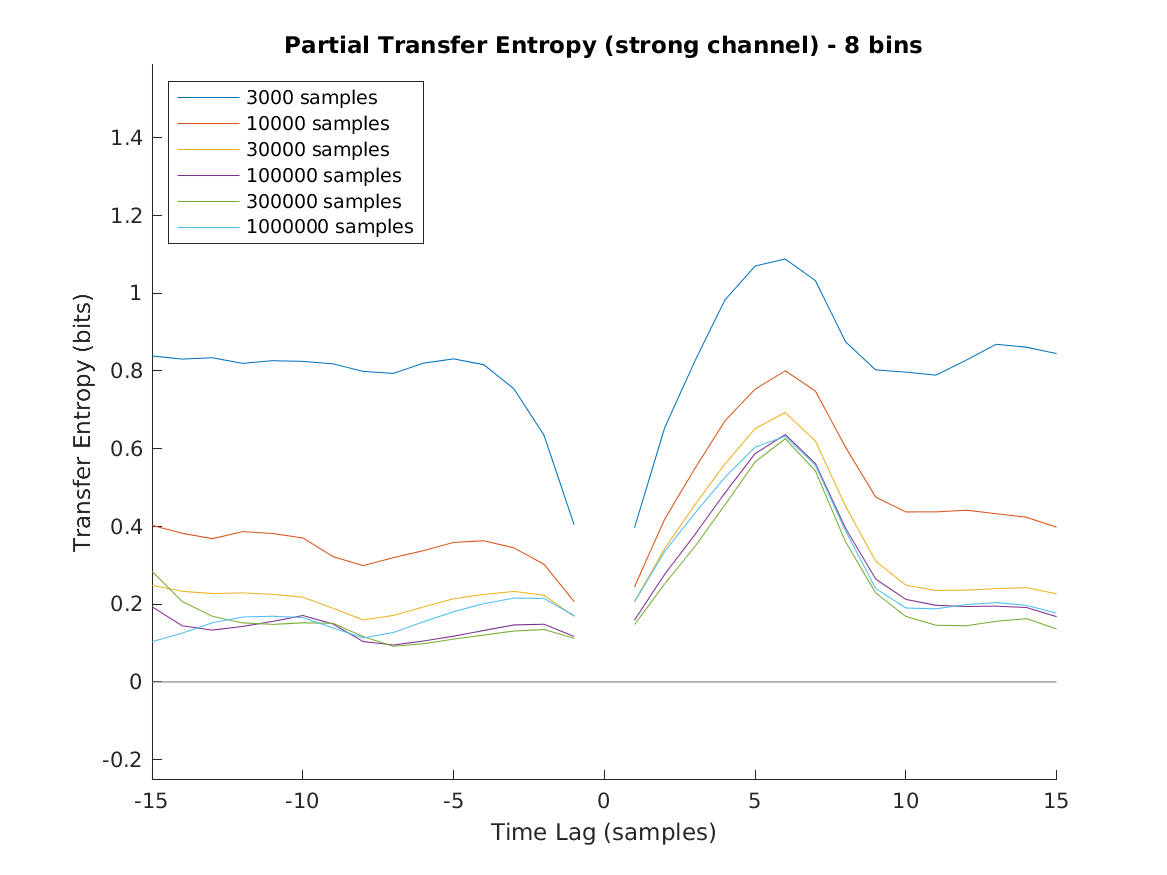
\includegraphics[width=5in]{plots/pte-strong-laglength-08bins.png}
%
\end{center}
%
\vfill
{\tiny \input{../LICENSE.md}}
%
\clearpage
%
%
% Front matter.
%
\pagestyle{plain}
\pagenumbering{roman}
\setcounter{page}{1}
%
\tableofcontents
%
\clearpage
%
%
% Document parts.
%
\pagestyle{plain}
\setcounter{page}{1}
\pagenumbering{arabic}
%
% FIXME - Guide NYI.
%% Chris's Entropy Library - User Guide - Overview
% Written by Christopher Thomas.

\chapter{Overview}
\label{sect-over}

This library provides a set of functions used for calculating entropy and
entropy-related measures on datasets. These were written to deal with
neuroscience data (continuous brain wave signals and discrete counts of
the numbers spike events seen), but the library should work with any type
of data.

Measures computed are:

\begin{itemize}
%
\item \textbf{Shannon Entropy} - The amount of ``surprise'' associated
with a given data sample, and the average ``surprise'' for samples in a
data stream. This is the information content of the stream.
%
\item \textbf{Conditional Entropy} - The amount learned from samples of
variable Y when we already know the value of a related variable X.
%
\item \textbf{Mutual Information} - The amount of information shared by
samples of related variables Y and X. Measuring either one gets you this
information.
%
\item \textbf{Transfer Entropy} - The amount of information about the
future of variable Y that you learn by knowing the past of variable X, in
addition to what you already know from the past of variable Y.
%
\end{itemize}

These measures are discussed in detail in Section \ref{sect-entropy}.

A brief description of how to use this library is given in Section
\ref{sect-howto}. For more information, see the sample code in the
``\verb|source-code|'' folder. This section also provides a brief overview
of considerations relating to neuroscience data analysis.

Section \ref{sect-extrap} describes the quadratic extrapolation algorithm
that was used in Palmigiano 2017. This is intended to allow reliable
estimates of several entropy measures with fewer data samples than would
otherwise be needed (or equivalently, to improve the reliability of these
measures using a fixed number of samples).

%
% This is the end of the file.

%\input{guide-model}
%% Chris's Entropy Library - User Guide - How-To Guide
% Written by Christopher Thomas.

\chapter{Using This Library}
\label{sect-howto}

\iffalse
A brief description of how to use this library is given in Section
\ref{sect-howto}. For more information, see the sample code in the
``\verb|source-code|'' folder. This section also provides a brief overview
of considerations relating to neuroscience data analysis.
\fi

%
% This is the end of the file.

%\input{guide-math}
%
%
\end{document}

%
% This is the end of the file.
